\section{Metodologia}

O modelo para reconfiguração do sistema de distribuição de energia elétrica, abordado nesse projeto, foi implementado na linguagem de de modelagem matemática (AMPL).

\subsection{Introdução a Linguagem de Programação Matemática}

O AMPL é uma linguagem de modelagem algébrica cuja função é descrever e resolver problemas a partir do seu modelo matemático. 
A linguagem fora desenvolvida nos ``Bells Labs'' por Robert Fourer, David Gay e Brian Kernighan com o intuito de ajudar as pessoas a comunicar modelos de otimização para sistema de computação, aproveitando o poder e a conveniência de formulações algébricas familiares \cite{ampl}. 
Possui, atualmente, suporte para uma grande diversidade de ``solvers'' tanto comerciais quanto códigos abertos .

\subsection{``Solvers'' comerciais}

Os ``solvers'' usados no AMPL, como dito anteriormente, podem ser tanto comerciais quanto constituídos de código aberto.
Ambos as categorias podem resolver determinados problemas de acordo com a natureza do sistema. 

\subsection{Hipóteses e definições da formulação do problema}

\begin{figure}[H]
    \centering
    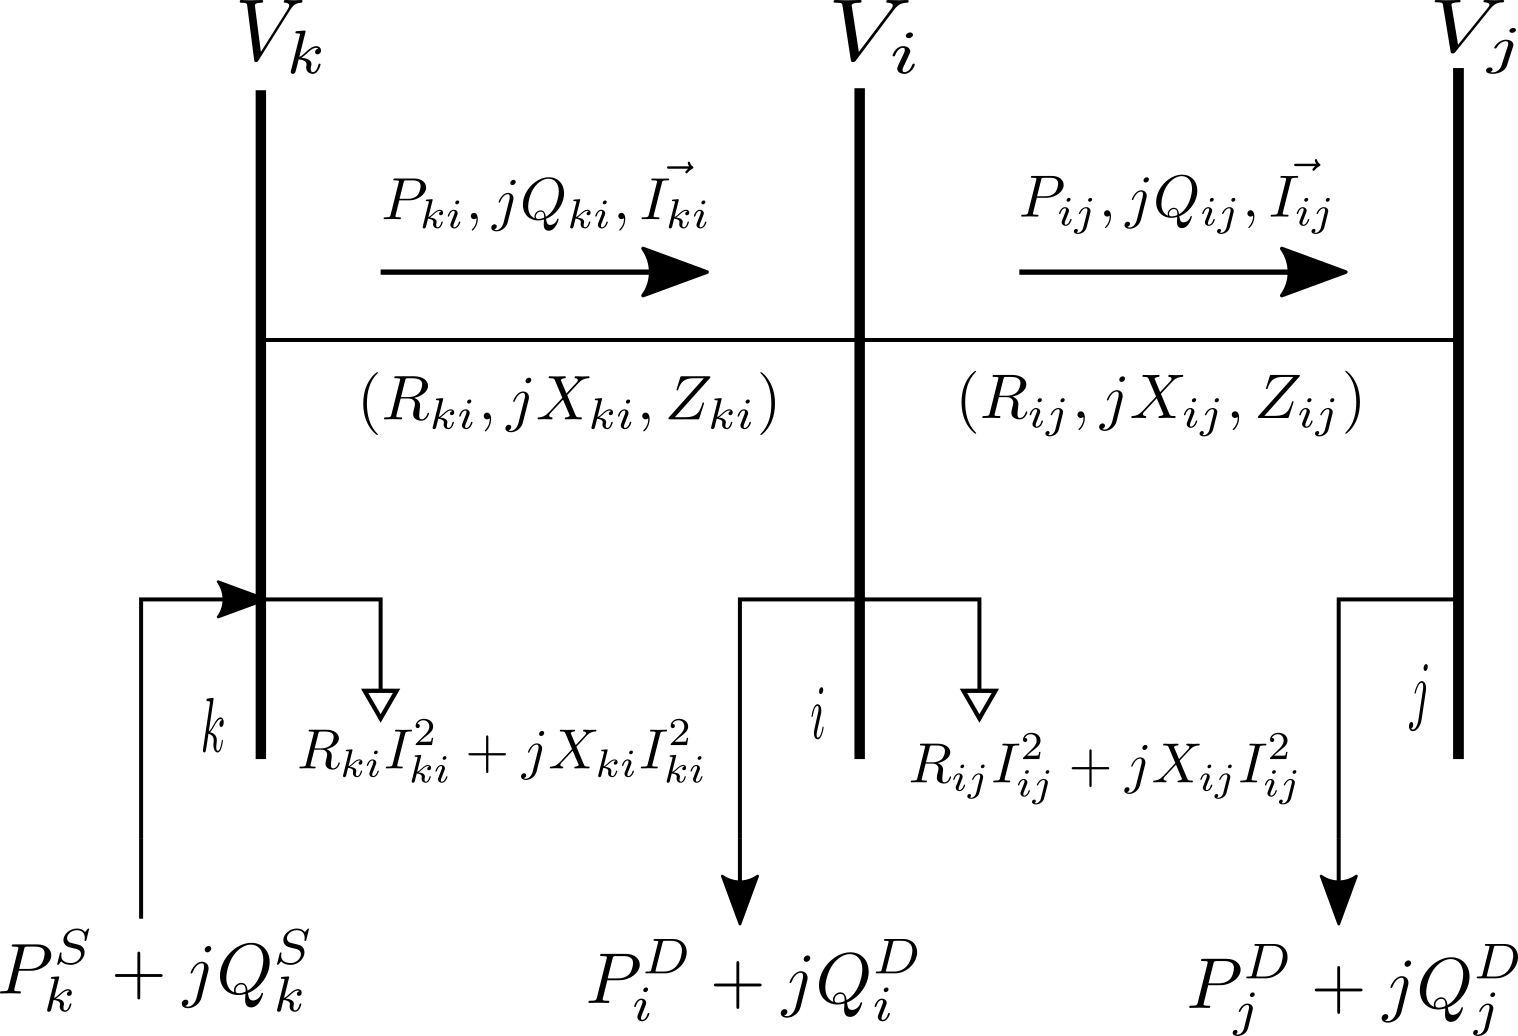
\includegraphics[scale = 1.2]{01_img/diagrama_nos.png}
    \caption{Sistema de distribuição radial}
    \label{fig:SDR}

\end{figure}

Hipóteses adotadas:
Visando representar o funcionamento em regime permanente de um sistema de distribuição de energia, são feitas as seguintes hipóteses (comumente usadas nas formulações de varredura de fluxo de carga \textbf{citar Shirmohammadi1988ANetworks} e mostradas na figura \ref{fig:SDR}.

\begin{itemize}
    \item As demandas nas cargas na rede de distribuição são representadas como potência ativa e reativas contantes;
    
    \item O sistema é balanceado e representado pelo seu equivalente monofásico;
    
    \item As perdas de potência ativa e reativa no circuito \textit{ij} estão concentradas no nó \textit{i}.
    
    \item As chaves são representadas como circuito curtos de impedância nula.
\end{itemize}

\subsection{Modelo de otimização}

O modelo de otimização interpretado pelo AMPL possui a seguinte forma:

{\raggedleft
\shadowbox{
\begin{minipage}{\dimexpr\textwidth-\shadowsize-2\fboxrule-2\fboxsep-8pt}
    
    \begin{center}
        Minimizar: Função objetivo        
    \end{center}

\hspace{2cm}Sujeito a:

    \begin{center}
        Restrições físicas\\
        Restrições operativas\\
    \end{center}
\end{minipage}
}}

As restrições do problema devem ser tais que modelem as leis da física que regem um sistema de distribuição de energia elétrica e as faixas com as quais essas grandezas podem operar ao longo da rede.
Para isso define-se dois conjuntos de restrições, restrições físicas e restrições operativas.

